\section{Noise removal}

Apart from artifact suppression, subspace methods can be further employed for the additional enhancement of the signal. The signal represented into a (\textbf{H}) Hankel data matrix could be seen as superposition of the $\hat{H}$ exact signal and the ($W$) pure noise. Taking into account that \textbf{wgn} is fully orthogonal to the signal to be estimated. Using an analogy of multivariate version of Pythagorean lemma for triangle, it is possible to recover the clean signal. Whereby the exact noise could be recovered via SVD as follow:


\begin{figure}[!htbp]
\minipage{0.5\textwidth}%
\centering
\begin{equation}
 \hat{H}=\hat{U}\hat{\Sigma}\hat{V^{h}}=[\hat{U_{1}} \hat{U_{2}}]
\begin{pmatrix}
 \hat{\Sigma_{1}}&0\\
 0&0
 \end{pmatrix}
 [\hat{V_{1}} \hat{V_{2}}]
 \end{equation}
\endminipage\hfill
\minipage{0.5\textwidth}%
\centering
 \begin{equation}\label{eq3}
 H=U \Sigma V^{h}=[U_{1} U_{2}]
\begin{pmatrix}
 \Sigma_{1}&0\\
 0&\Sigma_{2}
 \end{pmatrix}
 [V_{1} V_{2}] 
\end{equation}
\endminipage\hfill
\end{figure}

This estimation is possible under the fulfillment of the following conditions:
\begin{itemize}
    \item the clean signal is orthogonal to the noise $\hat{H^{T}}W=0$
    \item orthogonality of matrices $\hat{V_{1}}$ and $\hat{V_{1}}$ must be preserved in the inner product $\hat{V_{1}}W^{T}W\hat{V_{2}}=0$ \footnote{$W^{T}W=\lambda I$} 
    \item the smallest singular values $\sigma_{k}$ ins $\Sigma_{1}$ have to be larger than the largest noise singular value $\sigma_{K+1}$ in the $\Sigma_{2}$    
\end{itemize}

Noise separation performance depends critically on the the three criteria above, which in practice are never achieved, apart for the last condition. In order to satisfy the first criteria as the most important one it could be seen as an optimisation method. Minimizing the cost function in equation \ref{eq2} is completed by computing the transformation matrix $T$ such as:

\begin{equation}\label{eq2}
min||HT-\hat{H}||^{2}\rightarrow T=(H^{T}H)^{-1}H^{T}\hat{H}\rightarrow HT=H(H^{T}H)^{-1}H^{T}\hat{H}
\end{equation}

This estimation is known to be the minimum variance (MV) \cite{11} which gives the orthogonal projection $\hat{H}$ into the column space of $H$. Combining equations \ref{eq3} and \ref{eq2} the final estimation is equated as below:

\begin{equation}\label{eq5}
HT=UU^{T}\hat{H}=U_{1}U_{1}^{T}\hat{U_{1}}\hat{\Sigma_{1}}\hat{V_{1}^{T}}=U_{1}(\Sigma^{2}_{1}-\sigma^{2}_{w}I_{K})\Sigma_{1}^{-1}V_{1}^{H}=U_{1}(\Sigma^{2}_{1}-L\sigma^{2}_{v}I_{K})\Sigma_{1}^{-1}V_{1}^{H}
\end{equation}

Herein can be seen that the system is introducing a bias in the estimation as far as $U_{1}\neq\hat{U_{1}}$ and $\sigma^{2}_{v}=\frac{1}{L(M-K)}\sum_{i=K+1}^{M}\sigma_{1}^{2}$ is the average value of the noisy singular values. An outline of this algorithm could also be found in \ref{Ap3}. This method is a further improvement of Cadzow algorithm \cite{5} where the estimation is performed as $HT=U_{1}(\Sigma_{1})V_{1}^{H}$.

Apart from single channel method, multichannel Cadzow $MCC$ is also executed in here for comparative studies, where the NMR signals from different voxel locations are utilized \cite{14}. The voxels are the neighbours of the voxel of interest (VOI) which are located around into a horizontal cross-section. The method is also outlined in the section \ref{Ap31} adapted from \cite{13} and \cite{14}. This multichannel algorithm could further be enhanced (Multi-Channel Cadzow Enhanced (MCCE)) by taking into consideration different model order as well as different neighbouring size (3x3,5x5,7x7). In addition, different neighbour method is also investigated counting here square, diagonal and antidiagonal positioning. These four algorithm are executed on the data samples from NMR signal acquired in a human brain for 1024 voxels (32x32). 

In order to quantify the performance of each algorithm the signal-to-noise level is computed via equation:
\begin{equation}\label{SNR1}
SNR=20*\log\bigg\{\frac{var(Signal_{Filtered})}{var(Noise_{Residue})}\bigg\}
\end{equation} 
$Noise_{Residue}$ is the last 200 (arbitrary) sample of the filtered signal since in the FID case the main signal is at the beginning of the induction. Whereas the oscillation in the signal happening at the very end are considered noise since they do not came from any activity in the brain. 





\begin{figure}[!htbp]
\minipage{0.5\textwidth}%
\centering
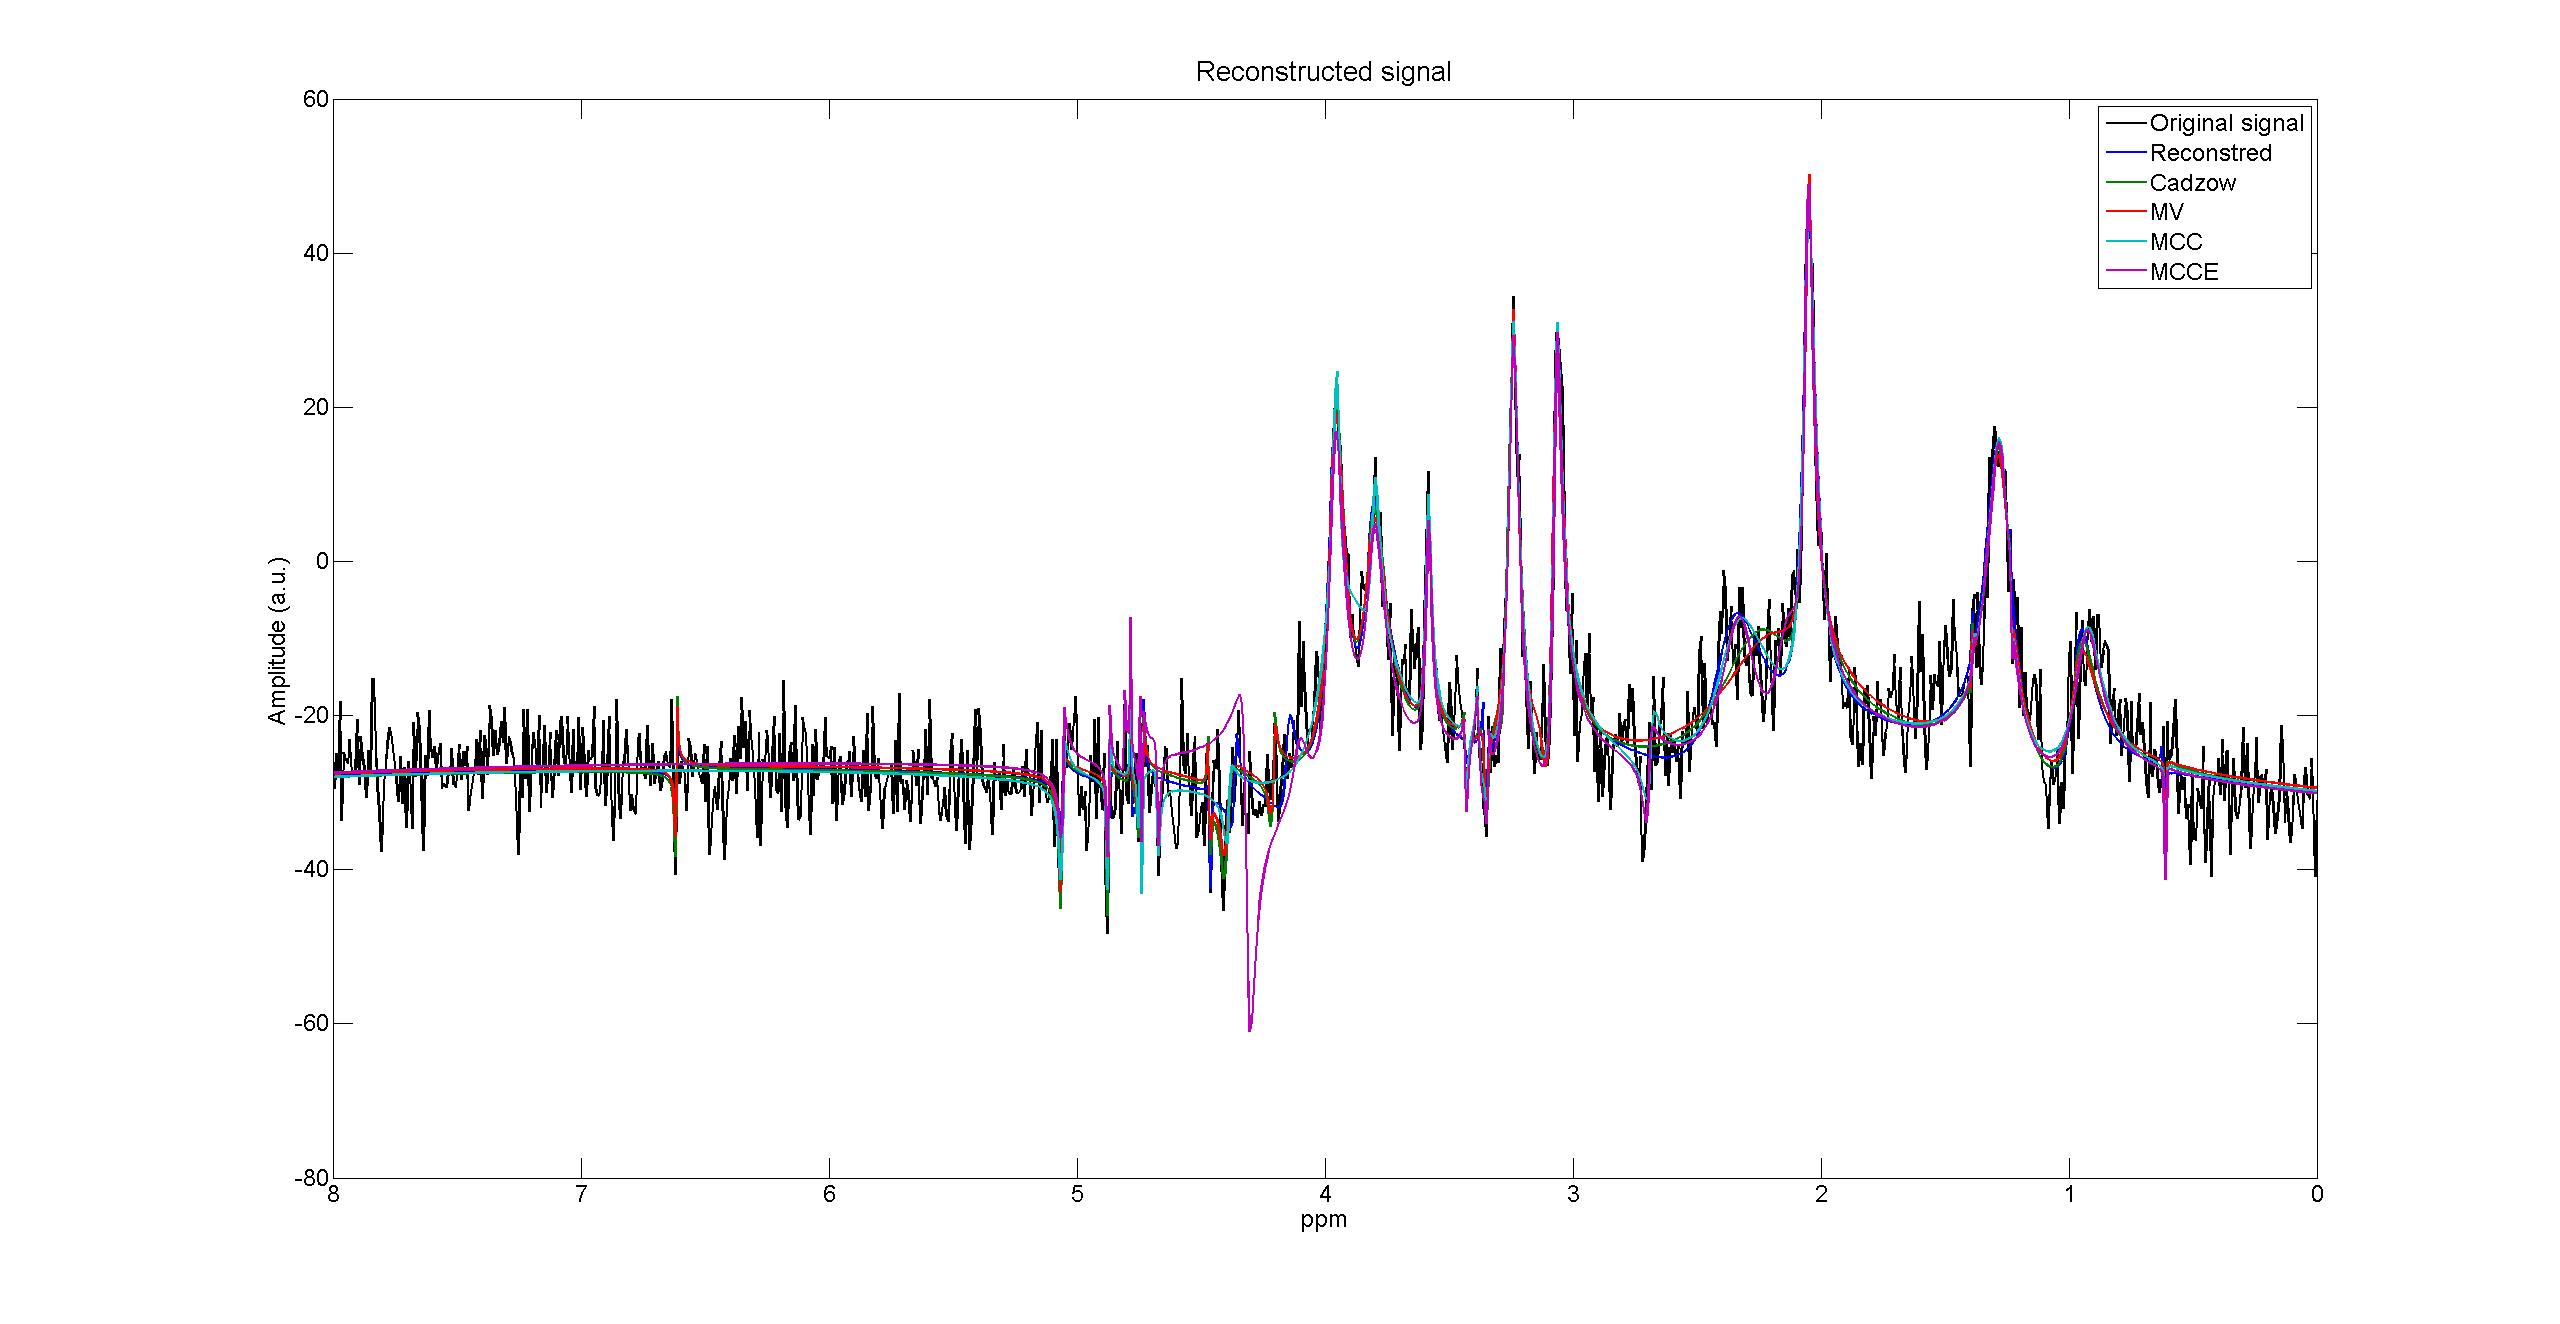
\includegraphics[width=1\textwidth]{final.jpg}
\subcaption{Reconstructed Signal}\label{Nadya12}
\endminipage\hfill
\minipage{0.5\textwidth}%
\centering
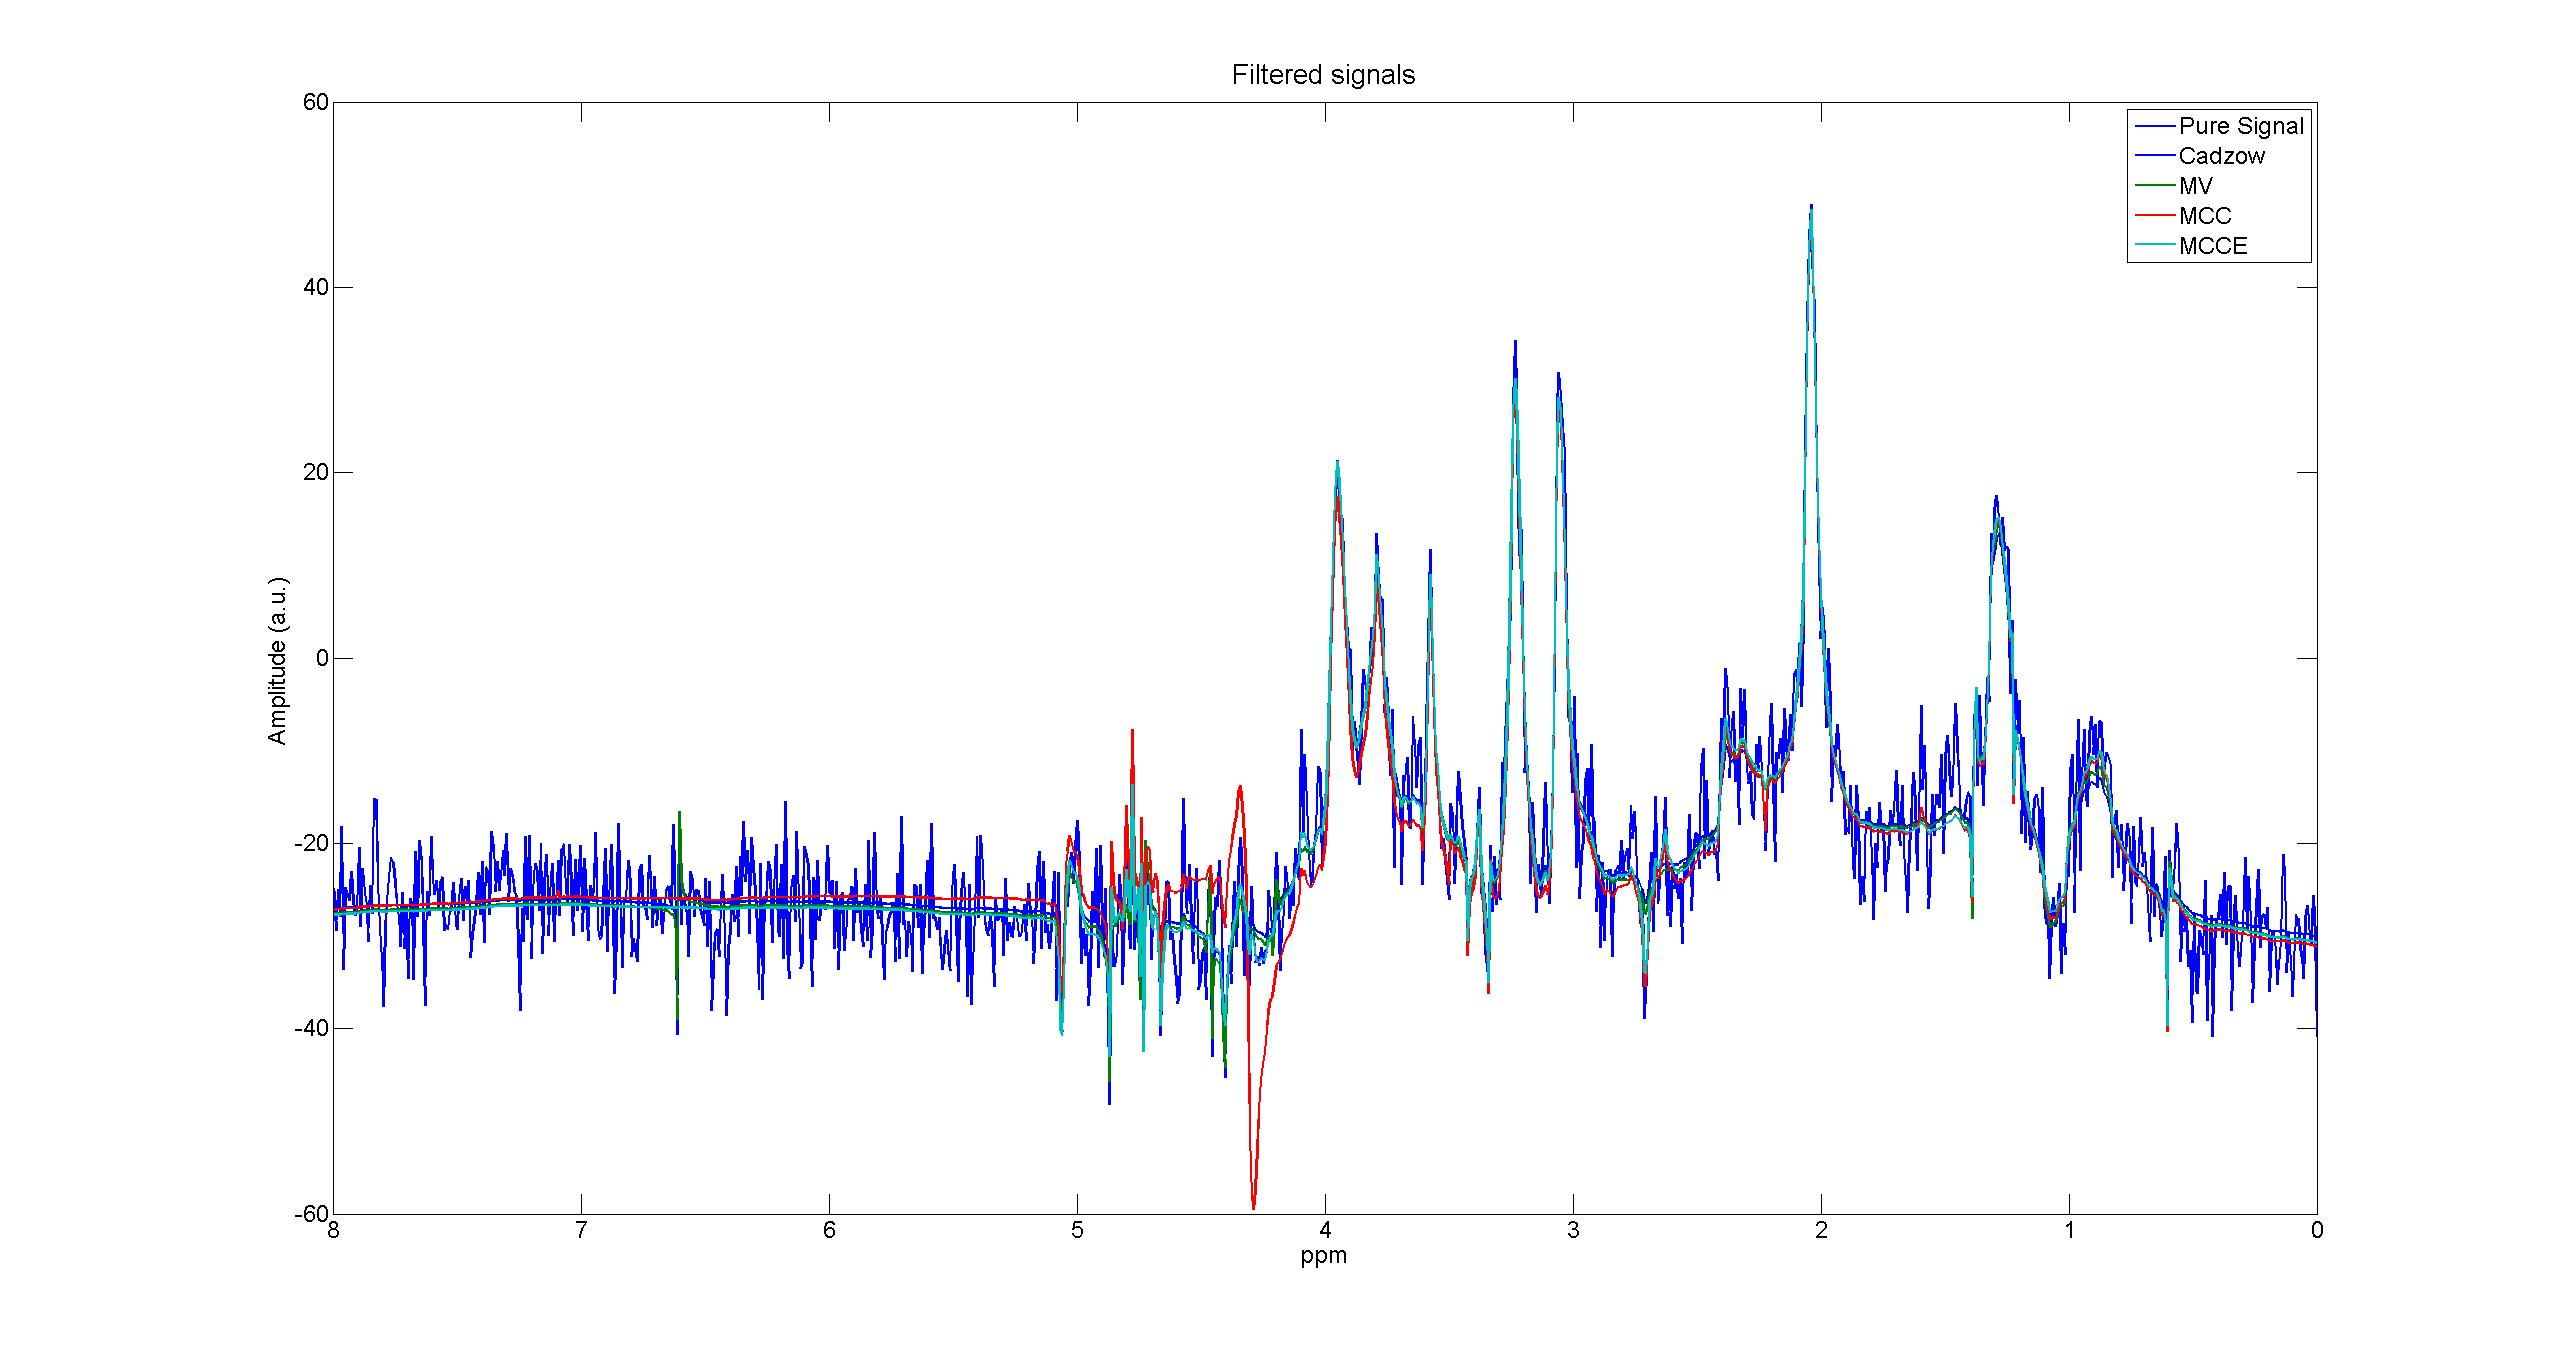
\includegraphics[width=1\textwidth]{final1.jpg}
\subcaption{Filtered Signal}\label{Nadya11}
\endminipage\hfill
\caption{Final results. }
\end{figure}


After removing the water component from all the signals at different voxels as in section \ref{sec1} the enhancement of the signal is performed via Cadzow, MV, MCC and MCCE and the results are outlined in figure \ref{Nadya11}. Furthermore, the parameter estimation for respective signal is performed using HTLS method as in the section \ref{sec2} and the table of values are listed in section \ref{Ap32}. Via the parameter estimated for each algorithm the reconstruction signal is obtained. The result of the reconstructed signal are drafted in figure \ref{Nadya12}. 





 \begin{table}[!htbp]
\centering
\caption{SNR evaluation for different methods}\label{tab11}

\begin{tabular}{c c c c c c} 
\hline 
$ $&$Signal$&$Cadzow$&$MV$&$MCC$&$MCCE$ \\
\hline 
$SNR$&$ 31.3230$&$ 61.2315$&$ 64.9762$&$ 68.9809$&$ 98.9809$\\
\hline 
\end{tabular}
\end{table}

As it is expected the SNR value increases after applying Cadzow as the first enhancement algorithm. The SNR is higher case of MV as compareD to Cadzow since the filtering of noise is higher due to the higher reduction of the principal singular values in equation \ref{eq5}. Furthermore, the multichannel algorithm yields better performance as compare to the both Cadzow and MV since it takes into account 3x3 neighbours. Overall, the MCCE outperforms the previous methods since it has been optimized over the three parameter models, model order, neighbouring distance and manner. The MCCE is indicated to have the best performance for model order of 26 over a neighborhood of 7x7 for in an square orthogonal manner.


\subsection{Cadzow vs Minimum Variance}

These methods are intrinsically quite similar to each other with the main difference that instead of computing the LS solution for the signal it does compute the minimum variance MV equation \ref{eq5}. Whereby the first criteria is better approximated with MV. In this way the separation of noise outperforms Cadzow algorithm since the orthogonality is much higher in the MV case thus the introduced bias is also lower \cite{11}. The SNR increases slightly for the MV case listed in the table \ref{tab11} and it provides much better results for the parameter estimation step. The closely spaced peaks are easier to be estimated via HTLS in case of the high SNR for the signal. Since the gap between the signal and the noise singular values is smaller in the MV case, the estimated parameters preserve better accuracy \cite{11} 

\subsection{Cadzow vs Multi-Channel Cadzow}

The very main difference between Cadzow and Multichannel Cadzow is that correlation between the channels can be fully exploited thereby a significant improvement of SNR has been observed in this case\cite{14}  as it is also testified in table \ref{tab11}. This is an important feature for multichannel data which enables the estimation of the common dynamics among the systems. Common dynamic among multichannel's means the same signal interfere throughout the voxels which is superimposed at different location in the brain at different phase and amplitude. This method is also estimated to be performed quite good at low spatial correlation of the NMR signal\cite{15}.

In this specific case the signal coming from one voxel will be intervened from the other surrounding voxels. However the scale of the correlation is different depending on the type of tissue which sit on the voxel and the geometrical distance between each voxel. In the Cadzow case this is not taken into consideration therefore the signal is significantly lower. 

In this case only one of the only one of the surrounding voxels is taken into consideration, meaning that this algorithm is totally  blind from the further tissues (neighbouring voxels). Nevertheless it outperforms the traditional Cadzow subspace algorithms. 

In multichannel approach, the signal of interest is approximated via a linear combination of the information coming from all the decomposed subspaces of the signal itself together with the other common subspace information coming from the other neighbouring voxels. Therefore, combination of this information will significantly enhance the signal  and therefore the unwanted signals are suppressed quite efficiently.  


\subsection{Cadzow vs Optimized Multi-Channel Cadzow }


A further improvement of the of the MCC is evidenced. As already stated, Cadzow is trying to suppress the noise into a single channel whereas MCCE attempt to provide the best performance possible.

At first the algorithm tries to observe the difference correlation between neighbours voxels along different direction. Whereby it considers only those specific voxels which contribute the most to the common dynamics. Unlike the simplest version of Cadzow, MCCE reveals that the vertically and horizontally voxels due to their proximity to the voxel of interest share much higher mutual information regarding the metabolite. 

After decomposition of this signals into different subspaces, the reconstructed signal takes into account the number subspaces where the information is correlated mostly to the voxel of interest. Consequently big amount of consistent information is explored and therefore the enhancement is far better compare to the simple Cadzow.

If the number of neighbourhood increases this means that the number of common dynamics event is also increased. Consequently the SNR of the final signal is testified to be higher. It is also totally not taken into account for the Cadzo algorithm. However, a high number of neighbouring voxels leads to much more heterogeneous tissues compared to the voxel of interest and thus will decay the performance of the MCCE.